\documentclass[12pt]{article}
%\usepackage[utf8]{inputenc}
%\usepackage[spanish,es-tabla]{babel}
\usepackage{polyglossia}
\usepackage{multirow}
\usepackage[T1]{fontenc}
\usepackage{mathptmx}
\usepackage{multicol}
\usepackage{amsmath}
\usepackage{float}
\usepackage{amssymb}
\usepackage{graphicx}
\usepackage{subfigure}
\usepackage{caption}
%\usepackage{subcaption}
%\usepackage{fourier}
\usepackage[left=1.5cm,right=1.5cm,top=2cm,bottom=2cm]{geometry}
\usepackage{fancyhdr} % Headers and footers
\pagestyle{fancy} % All pages have headers and footers
\fancyhead{} % Blank out the default header
\fancyfoot{} % Blank out the default footer
\fancyhead[L]{\small FCFM  2021} % Custom header text
\fancyhead[R]{\small UAdeC}
\fancyfoot[C]{\thepage} % Custom footer text

\setlength{\parindent}{0pt}

\usepackage{titlesec} % Allows customization of titles
\titleformat{\section}{\fontsize{14pt}{10pt}\bfseries}{\thesection.}{1em}{} % Change the look of the section titles
\titleformat{\subsection}{\fontsize{12pt}{10pt}\bfseries}{\thesubsection.}{1em}{}

\usepackage{abstract} % Allows abstract customization
\renewcommand{\abstractnamefont}{\fontsize{14pt}{10pt}\bfseries} % Set the "Abstract" text to bold

%----------------------------------------------------------------------------------------
%	TITLE SECTION
%----------------------------------------------------------------------------------------

\title{\vspace{-10mm}\fontsize{14pt}{10pt}\textbf{Tarea 6: ¿Qué nos dice que hagamos una ecuación diferencial?}} % Article title

\author{
\normalsize Jair Emmanuel Martinez Lopez\\ % Your name
\textit{\normalsize Facultad de Ciencias Físico Matemáticas - Universidad Autónoma de Coahuila}\\ % Your institution
\textit{\normalsize Enero 2021}\\
\textit{\normalsize jair\_ martinez@uadec.edu.mx} % Your email address
\vspace{-5mm}
}
\date{}

%----------------------------------------------------------------------------------------
\begin{document}
\maketitle
\thispagestyle{fancy}
%----------------------------------------------------------------------------------------
%    RESUMEN
%----------------------------------------------------------------------------------------

%----------------------------------------------------------------------------------------
%----------------------------------------------------------------------------------------
%    MAIN
%----------------------------------------------------------------------------------------
%\begin{multicols}{2} % Two-column layout throughout the main article text
\section*{Resumen}
Se han presentado ecuaciones del tipo
\begin{equation}
	\dfrac{dy}{dx}=f(x,y)
\end{equation}
En general, ninguna de las técnicas que has aprendido para resolver ecuaciones de primer orden ayudará a resolver una ecuación como la anteriormente presentada.\\
\\
Primero que nada, debe haber un lugar en el plano $x-y$ donde $f(x,y)$ está definida y tiene un valor único. Asumimos que existe una región rectangular $R$ en donde esto es verdadero. Si $y=y(x)$ es una solución, entonces debe ser diferenciable en todos los puntos dentro de $R$ y se sustituye en (1), entonces podrá ser identidad en $x$ para todas las $x$ in $R$. Así la solución $y=y(x)$ puede ser graficada como una curva en $R$. Supongase que camina a lo largo de la solución y se llega a un punto $P$ con coordenadas $(a,b)$. El siguiente paso es empezar a caminar tangente a la curva en $(a,b)$. Ahora, la dirección de la tangente en $(a,b)$, o mejor dicho la pendiente está dada por la derivada $\dfrac{dy}{dx}$ evaluada en $(a,b)$, usando (1), esta pendiente es, en efecto, $f(a,b)$.
\begin{center}
	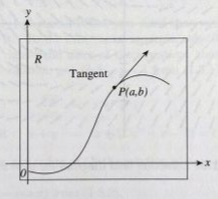
\includegraphics[scale=0.75]{Captura.PNG}
\end{center}
Esta pendiente puede ser especificada por un ángulo. Si la tangente a la curva $y=y(x)$ en $P$ hace un ángulo $\alpha$ con el eje $x$, entonces
\begin{equation}
	\tan \alpha = \left(\dfrac{dy}{dx} \quad en \quad P \right) = f(a,b).
\end{equation}
Ahora permitamos a $P(a,b)$ ser cualquier punto dentro de la región $R$. Se calcula $f(a,b)$ y el ángulo $\alpha$, y dibujar una corta línea empezando en $P$ y y extendiéndose en dirección de $\alpha$. Al seguir estos pasos se construye algo llamado "campo direccional" para la ecuación diferencial y muestra las diferentes soluciones posibles para esta misma [1].
%\end{multicols}
%----------------------------------------------------------------------------------------
%----------------------------------------------------------------------------------------
%    BIBLIOGRAFIA
%----------------------------------------------------------------------------------------
\section*{Bibliográfia}
\begin{enumerate}
	\item Computer Modeling: From Sports To Spaceflight ...From Order To Chaos, J. M. A. Danby
\end{enumerate}
%----------------------------------------------------------------------------------------
\end{document}